\section{Safety Plan}

\begin{figure*}[t]
    \begin{minipage}[t]{\textwidth}
        \centering
        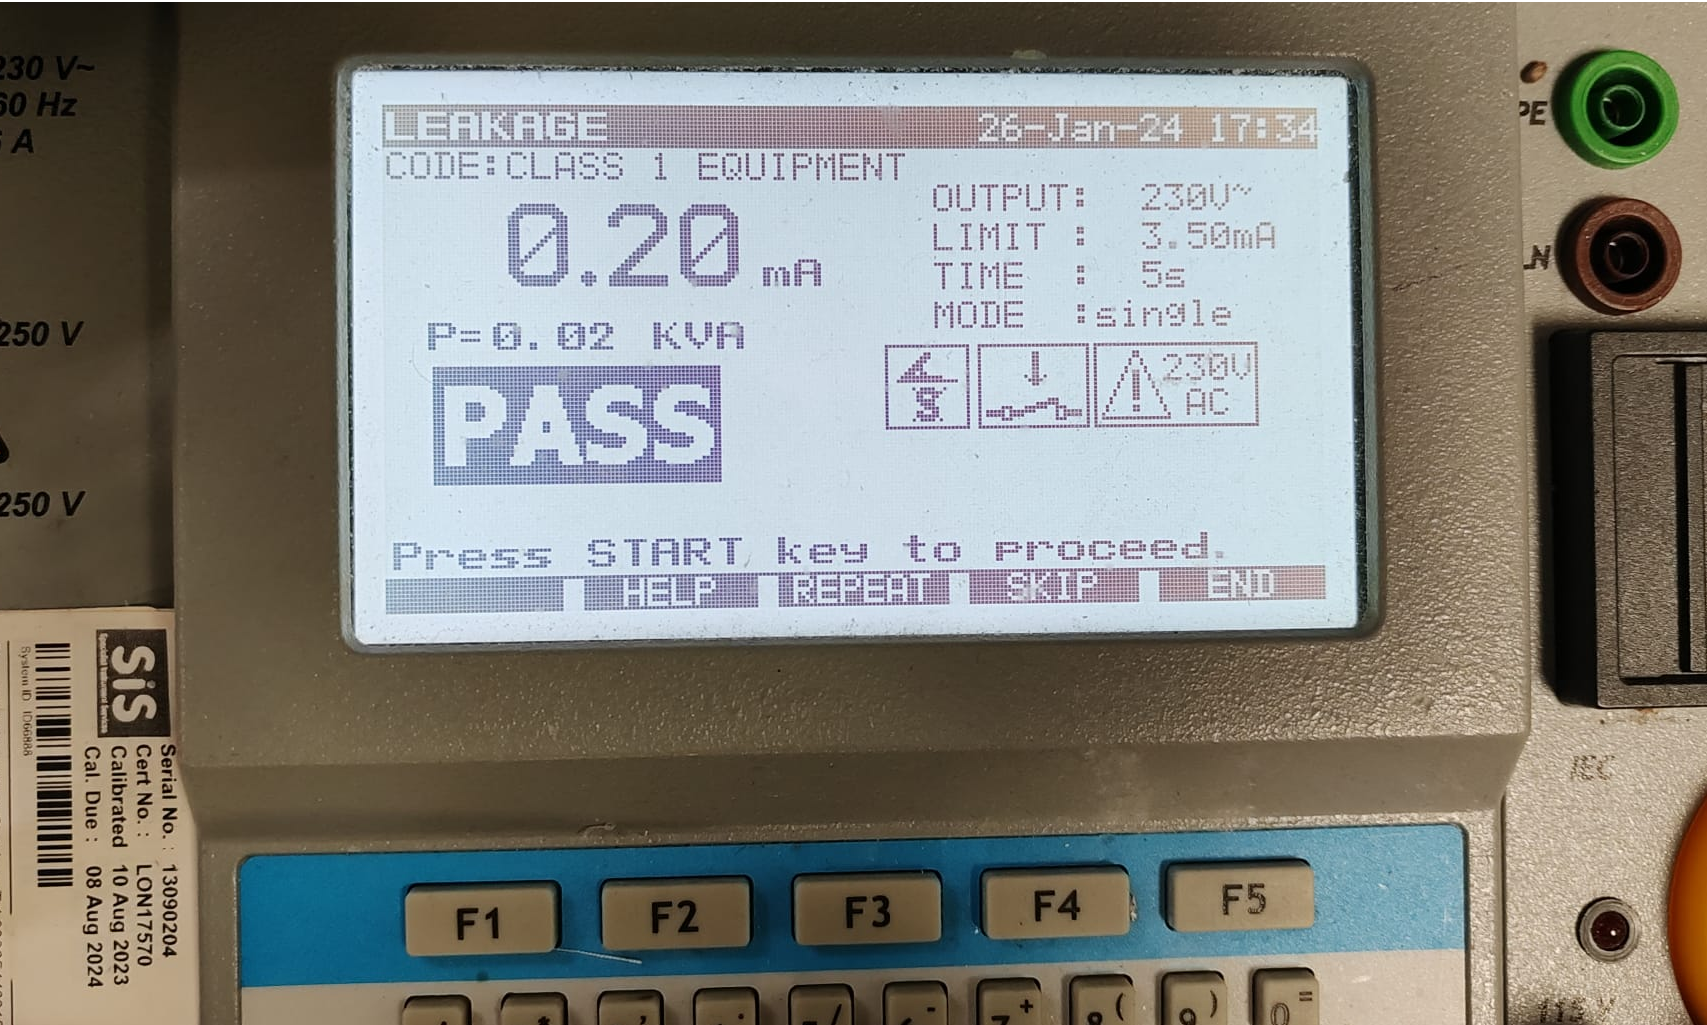
\includegraphics[width=\textwidth,height=8cm, keepaspectratio]{imgs/pattesting.jpeg}
        \caption{PAT Testing Machine}
        \label{fig:pat}
      \end{minipage}
      \hfill
  \end{figure*}
As the system is mechanical and electrical, many safety considerations need to be taken into account.
\subsection{Electrical Safety}
As mentioned in Section \ref*{sec:hardware} (Hardware), the system is powered by a 24V, 6.25A, 150W power supply, and must be stepped down to 5V for the Pi and 12V for the LED strip. This is achieved using an XL4015 Step Down Converter\cite{xl4015}, a variable step down converter that can output up to 75W.
Due to the potential of high-current carrying wires, the PSU has been enclosed in a 3D printed case, which prevents accidental contact with the PSU's terminals.

A standard IEC C14 power connector and an RS Pro Snap-In Fused Rocker Switch\cite{rsproc14switch} are used to connect the PSU to the mains power.
As the power supply is a 6.25A power supply, I have chosen a 6A fuse for the switch, which is the closest fuse rating to the power supply's
current rating. This ensures that the fuse will blow before the power supply is damaged, should there be a short circuit in the system.

For wiring the power supply and connecting the step-down converters, I have chosen 18AWG wire, which is rated for 17A\cite{18awgwire}, 
more than enough for the system's power consumption. The wire is securely crimped to the power supply using a crimping tool.

In addition, my power supply has been PAT tested by technicians in the Level 1 Labs and has been deemed safe for use.
PAT (Portable Appliance Testing) is a process by which electrical appliances are routinely checked for safety\cite{patwiki}\cite{patspec}.
The following table describes the PAT testing results for my power supply as well as a description of the tests performed.

\begin{table}[h]
    \centering
    {\fontsize{8pt}{11pt}\selectfont
    \begin{tabularx}{\columnwidth}{|@{\hspace{3pt}}>{\raggedright\arraybackslash}p{2cm}|@{\hspace{3pt}}>{\raggedright\arraybackslash}p{1cm}|@{\hspace{3pt}}>{\raggedright\arraybackslash}p{1.4cm}|@{\hspace{3pt}}>{\raggedright\arraybackslash}X@{\hspace{3pt}}|}
    \hline
        \textbf{Test} & \textbf{Result} & \textbf{Req} & \textbf{Description} \\ \hline
        Earth Continuity & 0.06$\Omega$  & $\leq$ 0.1$\Omega$ & Verifies the earth wire is connected. \\ \hline
        Earth Leakage & 0.2mA & $\leq$ 0.75mA & Ensure the touchable metal parts cannot cause harm. \\ \hline
        Insulation Resistance & 320M$\Omega$ & $\geq$ 1M$\Omega$ & Ensure wires are sufficiently insulated. \\ \hline
    \end{tabularx}
    }
    \caption{PAT Testing Results}
    \label{tab:pat}
\end{table}

As shown in Table \ref*{tab:pat} and Figure \ref*{fig:pat}, the power supply has passed all PAT tests and is safe for use.

\subsection{Mechanical Safety}
Currently, the system does not contain any moving parts, and as such, there are no mechanical safety considerations that need to be taken into account
for this stage. However, as mentioned in \ref*{sec:projectplan} Stage 2 requires the use of a conveyor belt system, and Stage 3 requires the use of a vibratory bowl feeder.
In this stage, mechanical safety will be a key consideration and will be discussed in the relevant sections in the final report.